\chapter{Capacité du camion infinie}

Dans tout ce chapitre, on considère un graphe circulaire $G = (V,E)$ à $n$ sommets et muni d'une orientation. On suppose en outre que $p=q$, c'est-à-dire que le point de départ et d'arrivé du camion sont identiques.
\\

Par soucis de concision, nous nommerons ``algorithme dans le cas linéaire'' l'algorithme permettant d'obtenir le premier mouvement de la solution optimale et le coût d'une telle solution dans le cas où le graphe est une ligne. Cet algorithme est décrit dans l'article \cite{Benchimol2011} en section 8. On rappelle qu'un tel algorithme est linéaire en le nombre de sommet.

\section{Algorithme d'obtention de la solution optimale}

On note $S_{min}$ la meilleure solution réalisable obtenue et on l'initialise avec une solution faisant deux fois le tour du graphe (donc de coût $2\sum_{e \in E}c_e$).
\\

\textbf{Données initiales.} Le graphe $G$ avec la répartition $\bs{x}$.

\begin{enumerate}
\item \uline{Pour chaque $e_o \in E$}\label{Ze0 nul}
  \begin{enumerate}
  \item Construire le graphe linéaire obtenu en supprimant l'arrête $e_0$ de $G$.
  \item Calculer le coût et le premier mouvement de la solution optimale $S$ à l'aide de l'algorithme dans le cas linéaire.
  \item Si $S$ est réalisable et si $\mbox{Coût}(S) < \mbox{Coût}(S_{min})$, remplacer $S_{min}$ par $S$.
  \end{enumerate}
\item \uline{Pour chaque $u \in V$}\label{Ze0 unitaire}
  \begin{enumerate}
  \item Aller de $p$ à $u$ dans le sens direct en ramassant tous les vélos sur les stations rencontrées.
  \item Retourner en $p$ dans le sens indirect et poser les vélos.\\
    On obtient \textbf{le graphe $G$ avec une répartition $\bs{x_1}$}.
  \item \uline{Premier cas :}\\
    \textbf{Données initiales.} Le graphe $G$ avec la répartition $\bs{x_1}$.
    \begin{enumerate}
    \item Construire le graphe linéaire obtenu en coupant au niveau de la station $p$ et tel que $p$ soit à droite et $q$ à gauche sur une station vide.
    \item Calculer le coût et le premier mouvement de la solution optimale $S$ à l'aide de l'algorithme dans le cas linéaire.
    \item Si $S$ est réalisable et si $\mbox{Coût}(S) < \mbox{Coût}(S_{min})$, remplacer $S_{min}$ par $S$.
    \end{enumerate}
  \item \uline{Deuxième cas :}\\
    \textbf{Données initiales.} Le graphe $G$ avec la répartition $\bs{x_1}$.
    \begin{enumerate}
    \item Construire le graphe linéaire obtenu en coupant au niveau de la station $p$ et tel que $p$ soit à gauche et $q$ à droite sur une station vide.
    \item Calculer le coût et le premier mouvement de la solution optimale $S$ à l'aide de l'algorithme dans le cas linéaire.
    \item Si $S$ est réalisable et si $\mbox{Coût}(S) < \mbox{Coût}(S_{min})$, remplacer $S_{min}$ par $S$.
    \end{enumerate}
  \end{enumerate}
\end{enumerate}

\begin{thm}
La solution $S_{min}$ retournée à la fin de l'algorithme précédent est une solution réalisable optimale et la complexité de l'algorithme est quadratique en le nombre de sommets du graphe.
\end{thm}

La suite de ce chapitre va permettre de montrer ce théorème.

\section{Conditions nécessaires pour qu'une solution réalisable soit optimale}

\subsection{Borne supérieure du coût de la solution optimale}

\begin{lem}\label{capacite infinie - borne sup cout}
\emph{Borne supérieure du coût de la solution optimale}\\
Si la capacité $C$ du camion est infine et si $p=q$, alors le coût d'une solution optimale du SSBP est strictement inférieur $\displaystyle 2\sum_{e \in E}c_e$.
\end{lem}

\begin{proof}
Il suffit d'aller de $p$ à $p-1$ dans le sens positif en prenant tous les vélos sur chaque station (y compris en $p$). Tous les vélos du modèle sont alors dans le camion et toutes les stations sont vides. Puis il suffit de revenir de $p-1$ à $p$ dans le sens négatif en posant sur chaque station le nombre de vélo nécessaire pour l'équilibrer.
\end{proof}

En pratique, une capacité infinie signifie que la capacité du camion est supérieure au nombre total de vélos sur le graphe.

\subsection{Parité des $z_e$}

\begin{prop}\label{parité des Ze}
Soit $G=(V,E)$ un graphe connexe. Si $p=q$, alors tous les $z_e$ ont la même parité.
\end{prop}

\begin{proof}
Comme $p=q$, la condition d'Euler est également vérifiée pour $p$. Donc $z(\delta(v))$ est paire pour tout $v \in V$.\\
Soit $e \in E$. Selon la condition d'Euler, $z(\{e, e+1\}) = z_e + z_{e+1}$ est paire. Donc $z_e$ et $z_{e+1}$ ont la même parité. Par une récurrence immédiate, tous les $z_e$ ont la même parité.
\end{proof}

\subsection{Restriction du nombre de passages sur une arête particulière}

\begin{prop}
On suppose que la capacité $C$ du camion est infine et que $p=q$. Soit $S$ une solution optimale du SSBP. Alors il existe une arrête $e_0 \in E$ tel que le camion passe au plus une fois par $e_0$.
\end{prop}

\begin{proof}
Par l'absurde, on suppose que pour tout $e \in E$, le camion passe au moins deux fois sur $e$. Alors le coût de la solution optimale est supérieur à $2\sum_{e \in E}c_e$ ce qui contredit le lemme \ref{capacite infinie - borne sup cout}.
\end{proof}

De cette proposition, on en déduit qu'il suffit de distinguer deux cas :
\begin{itemize}
\item \uline{il existe $e_0 \in E$ tel que le camion ne passe pas par $e_0$.}\\
Dans la partie \ref{Ze0 nul} de l'agorithme, on trouve pour chaque $e_0$ enlevé une solution optimale sous contrainte $z_{e_0} = 0$ et on garde la meilleure.
\item \uline{le camion passe au moins une fois par tous les sommets et il existe $e_0 \in E$ tel que le camion passe exactement une fois par $e_0$.}\\
On démontrera que dans la partie \ref{Ze0 unitaire}, on trouve pour chaque $e_0$ une solution optimale sous contrainte $z_{e_0} = 1$ et on garde la meilleure.
\end{itemize}

\subsection{Restriction du nombre de passages sur l'ensemble des arêtes}

\begin{prop}\label{Ze inf 3 - lineaire}
Soit $G=(V,E)$ un graphe linéaire. On suppose que la capacité $C$ du camion est infine et que $p$ et $q$ sont des extrémités du grapghe. Alors il existe une solution réalisable optimale telle que : pour toute arête $e \in E$, le camion passe au plus trois fois sur $e$.
\end{prop}

\begin{proof}
Les auteurs de l'article \cite{Benchimol2011} ont donné un algorithme et une formule pour calculer les $z_e$ d'une solution optimale particulière. Pour $e \in E$
\begin{gather*}
  z_e = \mbox{max}
  \bigg(
    \underbrace{ 2 \left\lceil \frac{x(U_e)-y(U_e)}{C} \right\rceil\ }_{\displaystyle \le 2 \mbox{ (car } C\mbox{ est infinie)} } +
    \underbrace{ \eta(p,q,U_e) }_{\displaystyle \le 1}\,,\,
    \underbrace{ \mu(p,q,U,\bs{x},\bs{y}) }_{\displaystyle \le 2}
  \bigg)
  \le 3
\end{gather*}
\end{proof}

\begin{lem}\label{Ze inf 3 - circulaire}
Soit $G=(V,E)$ un graphe circulaire. On suppose que la capacité $C$ du camion est infine et que $p=q$. Alors il existe une solution réalisable optimale telle que : pour toute arête $e \in E$, le camion passe au plus trois fois sur $e$.
\end{lem}

\begin{figure}[ht]
  \centering
  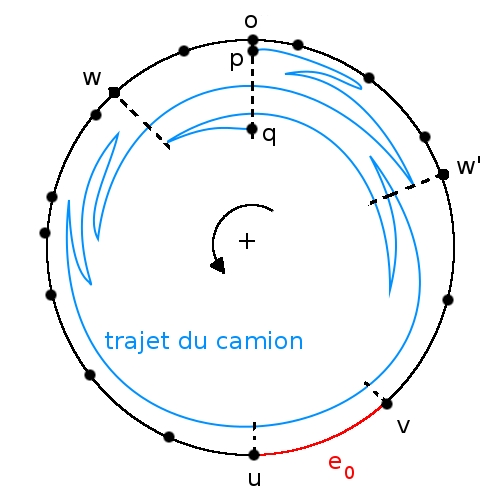
\includegraphics[scale=0.5]{GrapheCirculaire_PreuveZeInf3.jpg}
  \caption{Notations utilisées dans le cas du graphe circulaire avec une capacité infinie}
  \label{Notation graphe circulaire preuve Ze inf 3}
\end{figure}

\begin{proof}\uline{$1^{\mbox{er}}$ cas} : \uline{il existe $e_0 \in E$ tel que le camion ne passe pas par $e_0$.}

Pour $e_0 \in E$, selon la proposition \ref{Ze inf 3 - lineaire}, la solution optimale sous contrainte $z_{e_0}=0$ passe au plus trois fois par chaque arête.
\\

\uline{$2^{\mbox{ème}}$ cas} : \uline{le camion passe au moins une fois par tous les sommets et il existe $e_0 \in E$ tel que le camion passe exactement une fois par $e_0$.}

Soit $S$ une solution optimale sous contrainte $z_{e_0} = 1$. On note $o=p=q$ le point de départ et d'arrivée du camion. Quitte à changer l'orientation du graphe, on peut supposer que $e_0$ est parcourue dans le sens positif. et on note $u$ le sommet par lequel on entre sur $e_0$ et $v$ le sommet par lequel on sort de $e_0$. (cf figure \ref{Notation graphe circulaire preuve Ze inf 3} pour une synthèse des notations.)

Soit $w$ le sommet sur la portion $[o,u]_+$ le plus proche de $u$ et qui soit atteint par le camion après le parcours de $e_0$. Soit $w'$ le sommet sur la portion $[v,o]_+$ le plus proche de $v$ et qui soit atteint par le camion avant le parcours de $e_0$. Ces deux sommets sont bien définis car $o$ est atteint avant et après le passage sur $e_0$.

Alors, on peut toujours construire une solution optimale $S'$ comme suit :
\begin{enumerate}
\item\label{NewS1} démarrer en $o$.
\item\label{NewS2} aller jusqu'à $w'$ dans le sens négatif.
\item\label{NewS3} aller jusqu'à $w$ dans le sens positif en ramassant tous les vélos présents sur le chemin.
\item\label{NewS4} équilibrer la portion $[w,w']_+$ à l'aide de l'algorithme du cas linéaire en prenant :
  \begin{itemize}
  \item $p=w$ et $q=w'$
  \item $\displaystyle x_1(w) = \sum_{v \in E\left[ \left[w,w'\right]_+ \right]} x(v)$ et $y_1(w) = 0$
  \item $x_1(w') = 0$ et $\displaystyle y_1(w') = \sum_{v \in E\left[ \left[w,w'\right]_+ \right]} y(v)$
  \end{itemize}
\item\label{NewS5} aller jusqu'à $w$ dans le sens positif en équilibrant toutes les stations parcourues.
\item\label{NewS6} revenir en o dans le sens négatif.
\end{enumerate}
Il reste à démontrer que $S'$ équilibre bien le graphe et que $\mbox{Coût}(S') \le \mbox{Coût}(S)$.

\`A l'étape \ref{NewS4}, tous les vélos sont présent dans la portion $[w,w']_+$. La résolution à l'aide de l'algorithme du cas linéaire sur le graphe extrait $[w,w'[_+$ avec $p=w$ et $q=w'$ permet donc d'équilibrer la portion de graphe avec au plus trois passages sur chaque arête de $[w,w']_+$.

\`A la fin de l'étape \ref{NewS4}, les stations de la portion $]w,w'[_+$ sont équilibrées et celles de la portion $[w',w]_+$ sont vides et tous les vélos nécessaires pour l'équilibrer sont sur $w'$. L'étape \ref{NewS5} permet donc bien d'équilibrer les stations de $[w',w]_+$ et l'étape \ref{NewS6} de revenir en $o$. En outre, par construction de $w$ et $w'$ la solution $S$ passait au moins trois fois par chaque arête de $[w',w]_+$. Or $S'$ passe exactement trois fois par chaque arête de $[w',w]_+$.
\end{proof}